\documentclass[12pt]{article}
\usepackage{amsmath}
\usepackage{amsthm}
\usepackage{amssymb}
\usepackage{enumerate}
\usepackage{graphicx}
%\usepackage{fullpage}
\usepackage[top=1in, bottom=1in, left=0.8in, right=1in]{geometry}
\usepackage{multicol}
\usepackage{wrapfig}
\usepackage{units}
\usepackage{setspace}
\doublespacing

\setlength{\columnsep}{0.1pc}

\title{Ropes - Alternative String Representation}
\author{Leo Martel, Paul Martinez, Andy Moreland}
\date{\today}
\begin{document}

\maketitle
\vspace{-0.3in}
\rule{\linewidth}{0.4pt}

%%%%%%%%%%%%%%%%%%%%%%%%%%%%%%%%%%%%%%%%%%%

\section{Introduction}

In this paper we will discuss the Rope data structure, a data structure intended to serve as a more robust and more performant alternative to the tradtional String type offered in most languages.
The seminal paper regarding Ropes was written by Hans-J. Boehm, Russ Atkinson and Michael Plass in 1995.
We will provide an overview of their paper, beginning with their justification for Ropes in the first place.
We will continue with a more technical recap of the implmentation details and running time guarantees of a rope.
As an exercise we have implemented our own Rope and we will give some rough benchmark estimates comparing various operations.
Finally, in order to more easily show off the Rope data structure, we will discuss a visualization we created that allows one to actively interact with a Rope data structure and visualize its internal structure.

\section{Justification for Expanded String Type}

Boehm, Russ and Plass (BRP) begin their paper by discussing some of the faults of traditional string types and the various ways that they could be improved.
We will provide a brief summary of their points.

Before attacking `the traditional string type,' we must first define it.
This traditional string type we refer to is the crude fixed length arrays of characters offered
by languages such as C as Pascal.
We can usually access individual characters via some sort of array access and perform higher level operations such as concatenation or substrings through library functions.
Such implementations usually do not include any metadata along with the array (such as its length), and are usually mutable.

BRP list immutable strings as one of the characteristics of a more robust string type, noting that strings are often used to communicate between modules and thus one should be able to operate on a string without risk of modifying the original owner's copy of the string.

Additionaly, common string operations should be efficient. This is a natural desire, but BRP  note that particularly string concatenation and substring operations should run fast and not require excessive space.

Perhaps most critically, a more robust string type should be able to scale and handle extremely long strings while remaining performant. BRP mention the original vi editor which was unable to handle large files due to a line length limit, and joke that a "six-month-old child randomly typing at a workstation would routinely crash some older UNIX kernels due to a buffer size limitation."

\section{Implementation and Running Time}

In order for string concatenation to run quickly, a desireable implementation should not copy the strings, which naturally suggests storing a string as a tree of smaller literals, which will be what we call our Rope. As defined by BRP, the leaves of this tree will be \textit{flat} strings, the traditional raw character arrays, and internal nodes will represent the concatenation of their children. BRP note that because the leaf notes are immutable, a sequence of concatenation and substring calls could lead to many of these nodes being shared among multiple ropes, implying that the structure is techincally a directed acyclic graph. As they do, we will continue to refer to them as trees as we will be primarily considering only one rope at a time.

As a result of tree-storage structure and minor adjustments, we note that the following operations can easily be executed: arbitrary indexing, concatenation, substring and iteration.
The first three all take logarithmic time through the use of self-balancing trees and the third takes linear time. Though, due to immutability, tree-rebalances are more expensive due to the copying of concatenation nodes. Thus BRP recommended that tree-rebalances are done rarely and only explicitly. To keep the size of the rope from getting out of hand in the meatime, BRP recommedn the follwing approach:

\subsection{Concatenation}

A common use case for strings is continaully concatenation at one end. Thus whenever the right argument is a string literal, we would like to avoid growing the tree excessively. We can do this by accounting for two cases. One, if both arguments are string literals, we will simply combine them into a new string literal. Two, if the left argument is a concatenation node but its right child is a string literal, then we will combine the right child with the right argument to form a new string literal and then return a new concatenation node with the left child. In other cases we simply create a new concatenation node. These two rules make the case of continually appending to the end of a string very efficient.

\subsection{Substring}

When taking substrings

\section{Benchmarking}

We wrote some code.

\section{Visualization}

In order to better visualize how a rope structure may be built up, we set out to write a simple text editor whose backing store is a Rope. Text editors are one of the more commonly cited uses for Ropes, so it seemed fitting. Accompanying the editor is a tree structure displaying the current state of the rope's internal representation.

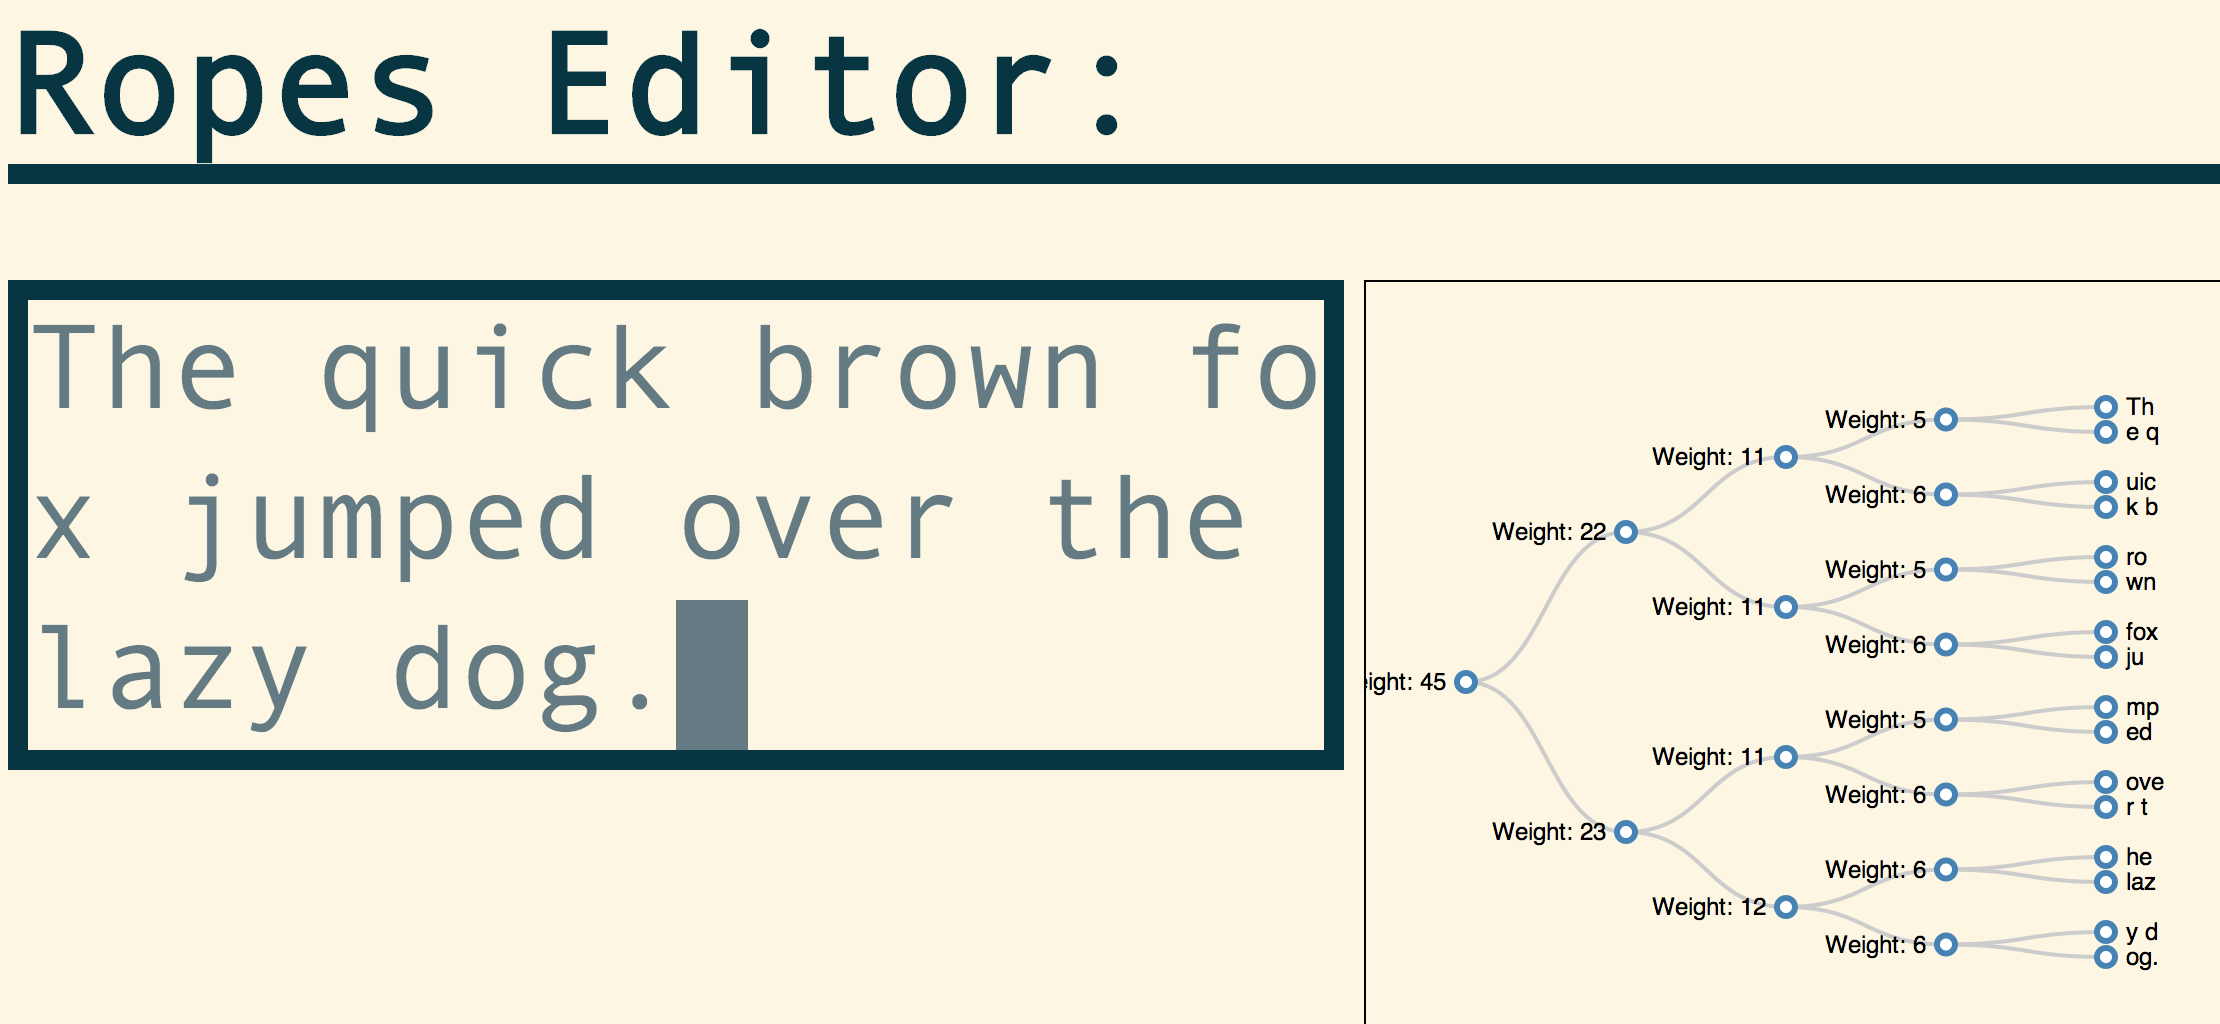
\includegraphics[scale=0.25]{editorImage1}

In building this simple demo, we began to consider some of the limitations of Ropes. While the immutability requirement may grant certain safety benefits, one could argue that it in a sense causes more trouble than it is worth. Consider a case where a large file has been build up via a series of sequential inserts at the end of the string. Then, when a character in the middle of the string is deleted. In the traditional implementation this first delete would require new concatenation nodes to be constructed all the way along the path from the root of the tree to node containing the edited string. Each subsequent insertion or deletion would continue to create a lot of work, including potentially memory allocations. In a text editor one often does a lot of local edits. It would be nice if a so-called `working-set' were located near the root of the tree. (We will ignore the fact that the bottleneck in most text editors these days is not the actual text manipulation but the neurons of the typist. We can still continue the exercise.)

One could use a splay tree for the this purpose, but then one completely forfeits some of the subtler niceties afforded by the immutability principle. For example, one could easily implmement an undo stack (very useful in a text editor!) by simply maintaining a list to previous representations of the file's string. Out of curiosity, we will forget this feature and continue to see what alterations we can apply. Suppose that in addition to having a completely mutable tree, we also had mutable string buffers. Then a series of local edits would splay a node up to the root, and as long as the buffer was moderately full every insert/delete would only take time proportional to the size of the buffer. This unfortunate fact means that this approach is unlikely to lead to any asymptotically better algorithms. We can see this by assuming that we have a block size of $b$. Though this hasn't been mentioned, supose we could somehow force each buffer to be at least half full. This would guarantee $\Theta(n/b)$ nodes in our tree, so splaying would take $O(\log n/b)$, but every individual operation at a node would also take $O(b)$ for a total time of $O(\log n/b) + O(b) = O(\log n) - O(\log b) + O(b) = O(\log n) + O(\log )$, which is nothing special. As long as $b$ on the order of $\log n$, then we won't lose any ground. Perhaps such a structure would be faster in practice due to the fewer allocations. As mentioned, insertions and deletions from the middle could force $O(\log n)$ new nodes per operation in the immutable rope, where as in this its $O(1 / \log n)$ allocations per insertion or deletion because you only would need a new node wheneve you add $\log n$ new characters! This is certainly better and likely indicates significant performace benefits.


\end{document}
